%Przykładowy plik ułatwiający złożenie projektu dyplomowego inżynierskiego.
%UWAGA: Generowany napis na stronie tytułowej o treści PROJEKT DYPLOMOWY INŻYNIERSKI został zaproponowany przeze mnie i nie jest, póki co, potwierdzony przez władze wydziału. Przed ostatecznym oddaniem tak złożonej pracy należy upewnić się jaka powinna być treść tego napisu. W momencie gdy uzyskam informację na temat treści tego napisu, dokonam niezbędnych zmian w źródłach.

\documentclass[eng,printmode]{mgr}
%opcje klasy dokumentu mgr.cls zostały opisane w dołączonej instrukcji

%poniżej deklaracje użycia pakietów, usunąć to co jest niepotrzebne
\usepackage{polski} %przydatne podczas składania dokumentów w j. polskim
%\usepackage[polish]{babel}%alternatywnie do pakietu polski, wybrać jeden z nich
\usepackage[utf8]{inputenc} %kodowanie znakĂłw, zaleĹĽne od systemu
\usepackage[T1]{fontenc} %poprawne składanie polskich czcionek

%pakiety do grafiki
\usepackage{graphicx}
\usepackage{subfigure}
\usepackage{psfrag}
\usepackage[polish]{babel}
\usepackage[utf8]{inputenc}
\usepackage{units}
\usepackage{lmodern}
\selectlanguage{polish}
%pakiety dodające dużo dodatkowych poleceń matematycznych
\usepackage{amsmath}
\usepackage{amsfonts}
\usepackage{upgreek}

%pakiety wspomagające i poprawiające składanie tabel
\usepackage{supertabular}
\usepackage{array}
\usepackage{tabularx}
\usepackage{hhline}

%pakiet wypisujący na marginesie etykiety równań i rysunków zdefiniowanych przez \label{}, chcąc wygenerować finalną wersję dokumentu wystarczy usunąć poniższą linię
\usepackage{showlabels}

%definicje własnych poleceń
\newcommand{\R}{I\!\!R} %symbol liczb rzeczywistych, działa tylko w trybie matematycznym
\newtheorem{theorem}{Twierdzenie}[section] %nowe otoczenie do składania twierdzeń

%dane do złożenia strony tytułowej
\title{Wyznaczanie kierunku przylotu sygnału akustycznego z zastosowaniem systemu mikrofonów}
\engtitle{Determination of the direction of acoustic signal arrival using a microphone system}
\author{Paweł Rachwalski}
\supervisor{dr inż. Bogdan Kreczmer. PWr, I-6}
%\guardian{dr hab. inż. Imię Nazwisko Prof. PWr, I-6} %nie używać jeśli opiekun jest tą samą osobą co prowadzący pracę

%\date{2008} %standardowo u dołu strony tytułowej umieszczany jest bieżący rok, to polecenie pozwala wstawić dowolny rok

%poniżej jest lista kierunków i specjalności na wydziale elektroniki, należy wybrać właściwe lub dopisać jeśli nie ma odpowiednich
\field{Automatyka i Robotyka (AIR)}
\specialisation{Robotyka (ARR)}
%\specialisation{Komputerowe sieci sterowania (ARK)}
%\specialisation{Systemy informatyczne w automatyce (ASI)}
%\specialisation{Komputerowe systemy zarzÄ…dzania \\procesami produkcyjnymi (ARS)}
%\field{Elektronika i telekomunikacja (EIT)}
%\specialisation{Akustyka (ETA)}
%\specialisation{Aparatura elektroniczna (EAE)}
%\specialisation{Elektroniczne i komputerowe \\systemy automatyki (ESA)}
%\specialisation{Zastosowania inĹĽynierii komputerowej \\w technice (EZI)}
%\specialisation{Inżynieria dźwięku (EID)}
%\specialisation{Elektronika stosowana \\i optokomunikacja (TEO)}
%\specialisation{Telekomunikacyjne sieci szerokopasmowe (TSS)}
%\specialisation{Teleinformatyczne sieci mobilne (TSM)}
%\specialisation{Sygnały w telekomunikacji cyfrowej (TSC)}
%\specialisation{Teleinformatyczne systemy rozsiewcze (TSR)}
%\field{Informatyka (INF)}
%\specialisation{Systemy informatyki w medycynie \\i technice (IMT)}
%\specialisation{InĹĽynieria systemĂłw informatycznych (INS)}
%\specialisation{InĹĽynieria internetowa (INT)}
%\specialisation{Systemy i sieci komputerowe (ISK)}
%\field{Teleinformatyka (TIN)}
%\specialisation{Teleinformatyka (TIN)}

%tutaj zaczyna się właściwa treść dokumentu
\begin{document}
\bibliographystyle{plabbrv} %tylko gdy uĹĽywamy BibTeXa, ustawia polski styl bibliografii

\maketitle %polecenie generujące stronę tytułową
\dedication{6cm}{Pracę tę dedykuję rodzicom, w podziękowaniu za wsparcie i wiarę w moje możliwości}

\tableofcontents %spis treści

%poniżej znajduje się przykładowa treść dalszej części dokumentu, zainteresowanych zachęcam do rozszyfrowania frazy "Lorem ipsum" :)
\chapter{Wstęp}
Wstępwstepepepepepepepepeppeepep

\chapter{Analiza problemu}
Źródłem dźwięku jest ciało wytrwarzające mechaniczną falę poprzeczną, fala ta może rozchodzić się tylko w ośrodkach sprężystych takich jak ciała stałe, ciecze i gazy. Mikrofon tak samo jak ludzkie ucho jest wrażliwy na ciśnienie akustyczne,  czyli zmienne w czasie odchylenie wartości ciśnienia statycznego panującego w ośrodku wywołane rozchodzeniem w nim fali akustycznej". %wikipedia
Źródła dźwięku można lokalizować i analizować za pomocą układów mikrofonowych oraz różnych metod. Poprawne rozwiąznie problemu zlokalizowania dźwięku polega na dobraniu odpowiedniego algorytmu lokalizacji oraz na poprawnym skonstruowaniu matrycy mikrofonów. 
 \newline




\section{TDOA}
Metoda Time Delay of Arrival(TDOA)jest często wykorzystywana w systemach lokalizacji źródła dźwięku ze względu na prostotę jej implementacji. Polega na zbieraniu próbek dźwięku i ich analizie, która odbywa się głównie w dwóch etapach. Pierwszym etapem jest identyfikacja opóźnienia czasowego próbek na różnych mikrofonach, opóźnienie to oznacza się symbolem $\tau$. Kolejny etap to obliczenie położenia źródła dźwięku na podstawie geometrii matrycy mikrofonów.
\begin{figure}[ht]

    \centering

  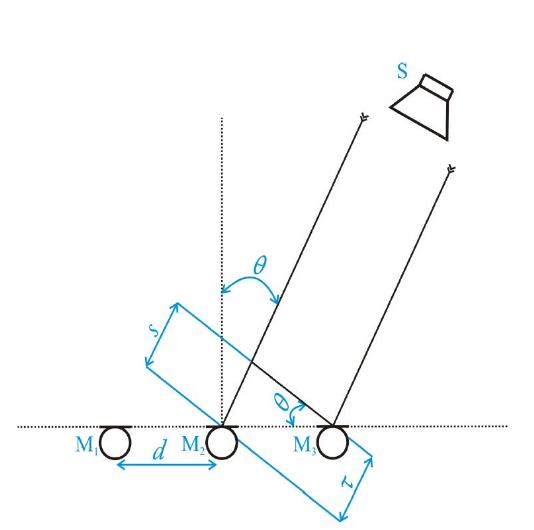
\includegraphics[width=0.5\textwidth, angle=0]{matryca.png}

    \caption{Liniowa matryca mikrofonów}

    

\end{figure}
\newpage Posiadając dane takie jak  opóźnienie synału oraz odległość miedzy mikrofonami, można wyznaczyć kąt $\theta$ za pomocą wzoru,
\begin{equation}
\theta = arcsin(\frac{\tau*V_{a}}{d}) 
\end{equation}
gdzie $\tau$ to opóźnienie sygnału, $V_{a}$ to prędkość sygnału w danym ośrodku, $d$ to odległość miedzy mikrofonami.

\section{Beamforming --- opóźnienie i sumowanie}
Metoda {\em beamforming} pierwotnie została stworzona na potrzeby kształtowania wiązki sygnału emitowanej przez nadajniki. Zauważono że może być ona wykorzystywana w przypadku odbiorników do przetwarzania danych pozyskancyh z matrycy czujników w celu wyznaczenia obrazu kierunkowego natężenia sygnału . Technika ta jest stosowana zarówno do ciągłego jak i dyskretnego rozkładu sygnału. Pozwala ona na budowe różnego typu matryc, w zależności od dostępnego sprzętu, pożądanej rozdzielczości przestrzennej oraz wrażliwości na wybrany kierunek. W porównaniu do metody TDOA {\em beamforming} wymaga wiele większej wydajności obliczeniowej. Konieczne też jest odpowiednie umieszcznie mikrofonów na matrycy, by uniknąć aliasingu przestrzennego.
\newline Tego niekorzystnego zjawiska można uniknąć jeśli różnica faz miedzy dwoma próbkowanymi sygnałami będzie mieściła się w przedziale wartości (-$\pi$,$\pi$), warunek ten jest spełniony gdy odległość miedzy czujnikami odpowiada nierówności:
\begin{equation}
 d <(\frac{s}{f_{max}}) 
\end{equation}

Najprostsze podejście związane z formowaniem wiązki sygnału opiera się na algorytmie DAS (Delay and Sum). W podejściu tym sygnały otrzymane z każdego z mikrofonów jest podawany na wejście osobnego bloku, który wprowadza odpowiednie opóźnienie. Otrzymane w ten sposób sygnały z wyjść wspomnianych bloków są sumowane. Układ taki określany jest mianem {\em beamformer} (patrz rys. \ref{fig-beamformer}).
\begin{figure}[ht]

    \centering

  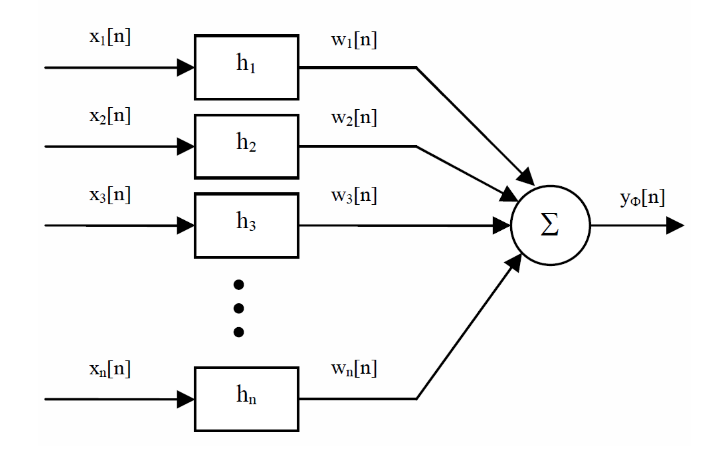
\includegraphics[width=0.5\textwidth, angle=0]{DAS.png}

    \caption{Schemat blokowy reprezentujący metodę DAS}
 \label{fig-beamformer}
    

\end{figure}
\newline 
Kierunek wyjścia wiązki $y_{\Phi}[k]$ jest określony w dziedzinie czasu przez zestaw wag $h_{i}$:
\begin{equation}
 y_{\Phi}[k] = \sum_{i=1}^n x_{i}[k-h_{i}(\phi)] 
\end{equation}
Gdzie $x_{i}[n]$ jest sygnałem odebranym przez mikrofon a $h_{i}(\Phi)$ jest opóźnieniem dla charakterystyki kierunkowej kąta.
Wartość RMS dla charakterystyk kierunkowych kąta oblicza się ze wzoru:
\begin{equation}
 V_{RMS}[\phi] = \sqrt{\frac{1}{N}\sum_{i=1}^N y_{\Phi}[i]^2 }
\end{equation}
Maksymalna wartość wyjścia RMS beamformera determinuje kąt pod którym znajduję się źródło dźwięku:
\begin{equation}
 \alpha = argmax(V_{RMS}[\phi])
\end{equation}
 Upraszczając przebieg algorytmu wygląda w sposób następujący:
 \begin{itemize}
\item Rejestracja sygnału.
\item Sumowanie opóźnień odpowiadająccych zmianie położenia względem położenia referencyjnego. 
\item Sumowanie przebiegu dla każdego sygnału.
\item Utworzenie funkcji korelacji oraz znalezienie jej maksimum które odpowiada szukanemu przez nas kątowi.
\end{itemize}

\chapter{Specyfikacja projektu}
System składa się z trzech bloków:
\begin{itemize}
\item Blok matrycy czterech mikrofonów.
\item Blok odpowiedzialny za wygenerownie i filrację obwiedni sygnału. 
\item Blok mikrokontrolera.
\end{itemize}
\section{Matryca mikrofonów}
Projekt nie przewidywał budowy matrycy mikrofonów wraz z konstrukcją toru wzmocnienia, dlatego zdecydowano się na zakup gotowego rozwiązania. Na rynku dostępny jest duży wybór czujników mikrofonowych wraz z dedykowanymi układami wzmaczniaczy, dwa z nich zdawały się być najbardziej odpowiednie.\\
Pierwszym z nich jest detektor dźwięku SEN-14262 produkowany przez firmę SparkFun[Rysunek 3.1], posiada on mikrofon elektretowy o zakresie częstotliwości od \unit[100]{Hz} do 10000Hz. Za wzmocnienie sygnału mikrofonowego odpowiada układ LMV324 z możliwością zmiany wzmocnienia od 20dB do 60 dB, podstawowo wartość ta jest usatwiona na 40 dB. Cały moduł posiada aż trzy niezależne wyjścia:
\begin{itemize}
\item Audio -- analogowy sygnał audio,
\item Envelope -- analogowy sygnał umożliwiający pomiar amplitudy sygnału,
\item Gate -- sygnał cyfrowy pozwalający na detekcje przekroczenia ustalonego poziomu amplitudy.
\end{itemize}

\begin{figure}

    \centering

  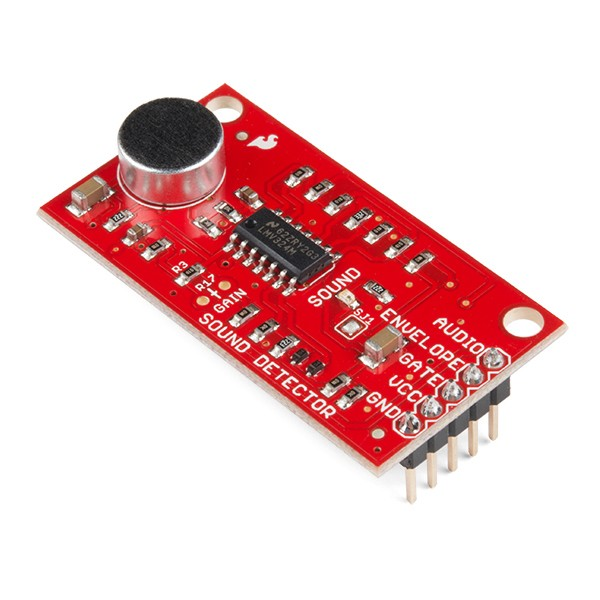
\includegraphics[width=0.33\textwidth, angle=0]{detektor1.jpg}

    \caption{SparkFun SEN-14262}

    

\end{figure}


 Drugie rozwiązanie to moduł czujnika dźwięku ze wzmaczniaczem MAX9814 produkowany przez firmę Adafruit[Rysunek 3.2], w jego skład wchodzi mikrofon elektretowy umożliwiający pomiary w zakresie 20Hz-20000Hz. Tor wzmacnienia czujnika jest oparty o układ MAX9814, który oferuje takie możliwości jak:
\begin{itemize}
\item AGC (Auto Gain Control) czyli automatycznie zmienne wzmocnienie zależne od poziomu natężenia sygnału wejściowego.
\item Zmienne maksymalne wzmocnienie sygnału 40, 50, 60dB. 
\item Ustawienie współczynnika Attack/Release 
\item sygnał wyjściowy na poziomie 2 Vpp
\end{itemize}
\newpage
\begin{figure}

    \centering

  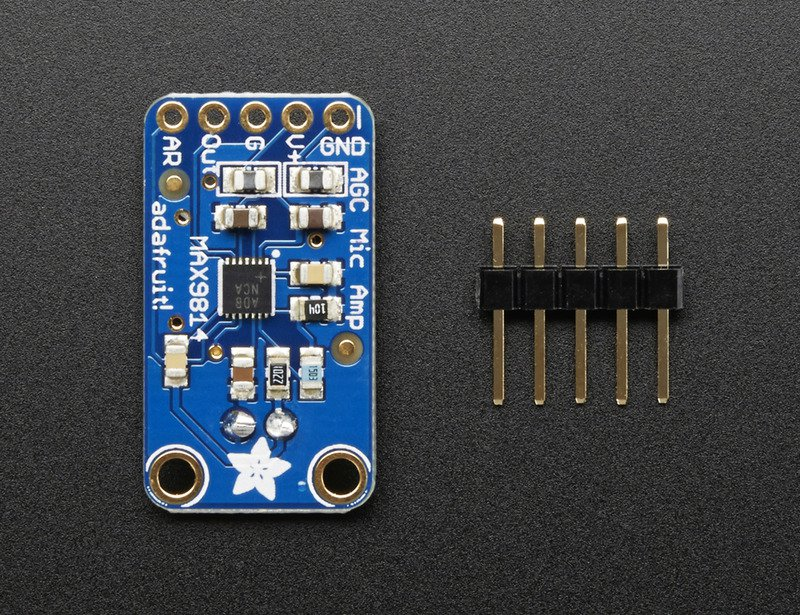
\includegraphics[width=0.33\textwidth, angle=0]{detektor2.jpg}

    \caption{Adafruit MAX9814}

    

\end{figure}

Ostatecznie wybrano rozwiązanie zaproponowane przez firmę Adafruit, ze względu na automatyczną kontrolę wzmocnienia, możliwość regulowania współczynnika Attack/Release oraz o wiele korzystaniejszą wartość współczynnika zawartości harmonicznych THD który w układzie MAX9814 dla częstotliwości 1kHz plasuje się na poziomie poniżej 0,1\%, dodatkowo MAX9814 posiada o wiele niższą gęstość szumów.
\section{Generator obwiedni}
Czujnik firmy Adafruit nie posiada wyjścia umożliwiającego pomiar amplitudy. Dlatego też konieczne jest skonstruowanie zewnętrznego układu odpowiadającego za generowanie obwiedni. Rozwiąznie to podyktowane jest chęcią pominięcia złożonych obliczeń na mikrokontrolerze związanych z tranformatą Hilberta. Zastosowano prosty detektor obwiedni.
\begin{figure}

    \centering

  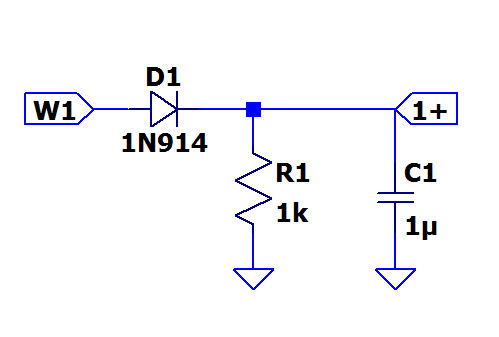
\includegraphics[width=0.6\textwidth, angle=0]{obwiednia.png}

    \caption{Schemat detektora obwiedni}


\end{figure}
\newpage
\noindent Dioda umożliwia przepływ prądu tylko jeśli zacisk wejściowy ma potencjał wyższy niż zacisk wyjściowy, kondensator gromadzi ładunek na zboczu narastającym następnie powoli uwalnia go przez rezystor gdy wzgórze opada co w efekcie pozwala uzyskać  filtr dolnoprzepustowy. Do zbudowania układu użyto diody 1N914 ze względu na jej dużą szybkość przełączania i wysoką przewodność. 
\section{Mikrokontroler}
Kolejnym krokiem przetwarzania sygnału uzyskanego z matrycy mikrofonów jest jego spróbkowanie oraz konwersja do postaci cyfrowej. 
Chcąc nie zwiększać ilości elementów w układzie elektronicznym zdecydowano się na zastosowanie przetwornika ADC który będzie jednym z peryferiów mikrokontrolera. Przy projektowaniu systemu brano pod uwagę głównie mikrokontrolery firmy STM32 ze względu na to, że dostępne są:
\begin{itemize}
\item aplikacja CubeMX, która generuje szkielet projektu i przyśpiesza pracę związane z konfiguracją mikrokontrolera,
\item wiele darmowych narzędzi oraz przejrzyste IDE SW4,
\item biblioteka HAL ułatwiajacą pracę z peryferiami,
\item aplikacja STM Studio, która umożliwa proste debuggowanie.
\end{itemize} 
Poszukiwania zawężono do mikrokontrolerów z rodziny F4, ponieważ są one oparte na rdzeniu CortexM4 pozwalającym na szybką pracę z jednostkami zmiennoprzecinkowymi oraz szybkie obliczenia dzięki wysokiemu taktowaniu rdzenia. Finalnie wybór padł na jednostkę STM32F446RET6, jej zalety szczególnie przydatne przy danym projekcie to:
\begin{itemize}
\item Częstotliwość taktowania do 180MHz.
\item Trzy przetworniki ADC o rozdzielczości 12 bitów.
\item 16--strumieniowy kontroler DMA.
\item 6 interfejsów UART, które pozwolą na jednoczesne monitorowanie każdego z mikrofonów przy przeprowadzaniu testów.
\item 128kB pamięci RAM.
\end{itemize} 
\chapter{Projekt i realizacja modułu
 kierunku przylotu sygnału akustycznego}
 
 \section{Założenia działania modułu}
  Moduł został zaprojektowany, tak by mógł składać się z trzech oddzielnych członów opisanych we wcześniejszym rozdziale. Zasadę ich wspólnego działania opisuje schemat blokowy przedstawiony na rys. \ref{fig-schematblokowy}.
  \begin{figure}[!ht]

    \centering

  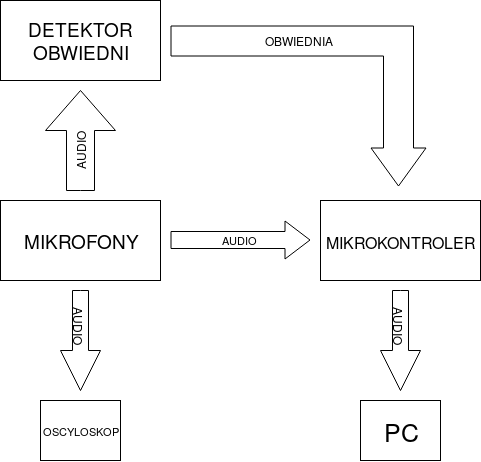
\includegraphics[width=0.5\textwidth, angle=0]{diagram.png}

    \caption{Schemat blokowy modułu}
 \label{fig-schematblokowy}
    

\end{figure}
%
Wzmocniony sygnał audio pochodzący z mikrofonów zostaje podany na wejście mikrokontrolera i detektora obwiedni. Dodatkowo możliwe też jest bezpośrednie podłączenie do układu oscyloskopu, który jest pomocny podczas fazy testowej modułu. Wyjście detektora obwiedni podłączono do mikrokontrolera. Dane z mikrokontrolera wysyłane są za pomocą interfejsu UART. Sygnały tego interfejsu przekierowane są do układu MAX232, który do komunikacji z komputerem udostępnia interfejs USB. Porównanie sygnałów audio otrzymanych przez mikrofony oraz mikrokontroler posłuży do sprawdzenia poprawności działania układu. 
\section{Schemat oraz płytka PCB}
Do zaprojektowania schematu elektronicznego oraz płytki PCB zostało użyte oprogramowanie KiCad.
\subsection{Sekcja zasilania}
Moduł został zasilony napięciem stałym 5V pochodzącym z zewnętrznego zasilacza sieciowego. Jednak z uwagi na to że mikrokontroler oraz systemy  mikrofonowe powinny zostać zasilone napięciem 3,3V, do modułu zaimplementowano stabilizator liniowy LM1117(patrz rys. \ref{fig-stabilizator}).
\begin{figure}[ht]

    \centering

  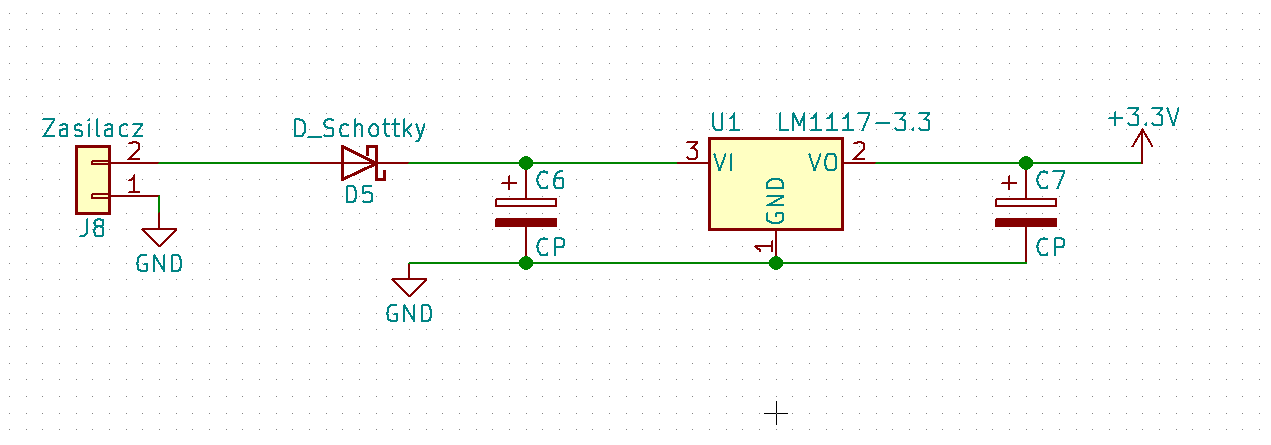
\includegraphics[width=0.7\textwidth, angle=0]{zasilanie.png}

    \caption{Stabilizator liniowy}
 \label{fig-stabilizator}
    

\end{figure}

W projekcie pominięto zabezpieczenie przed odwrotną polaryzacją źródła zasilania, ponieważ użyta wtyczka zasilacza nie pozwala podłączyć zasilania odwrotnie.

\subsection{Sekcja mikrofonów}
Ze względu na fakt, że mikrofony znajdują się na gotowych komercyjnych PCB , zostaną one przylutowane do płytki głównej poprzez goldpin. Zasilane są one napięciem 3,3V (patrz rys. \ref{fig-mikrofony}).
\begin{figure}[ht]

    \centering

  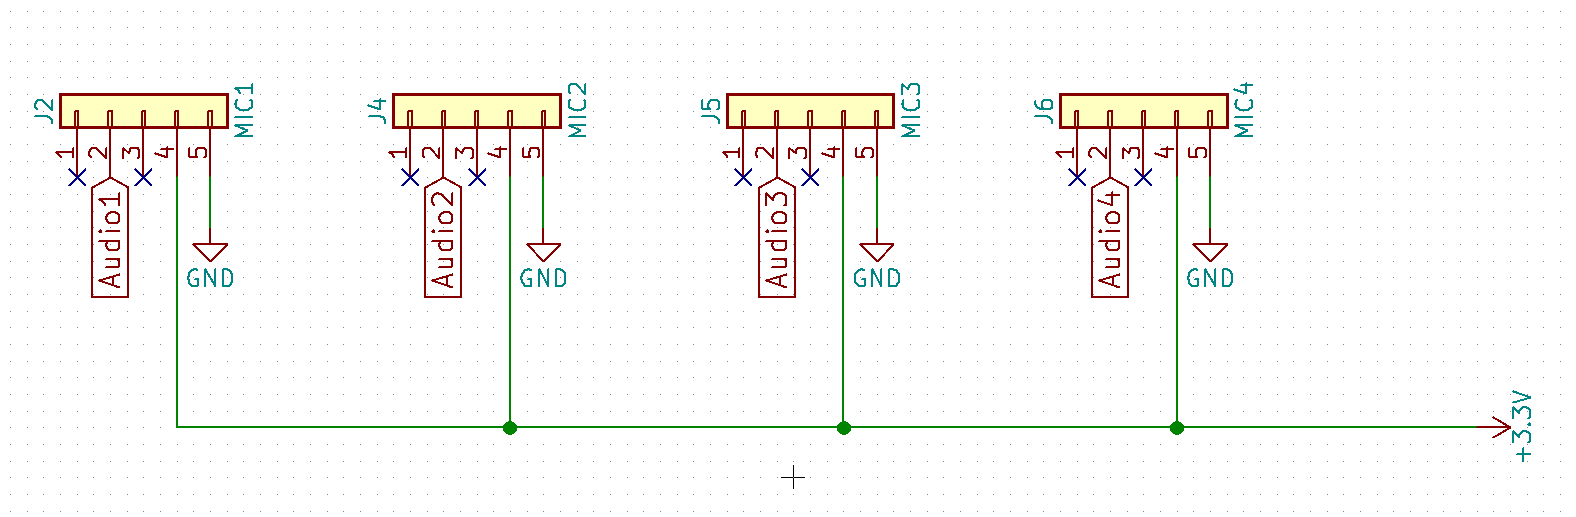
\includegraphics[width=0.9\textwidth, angle=0]{mikrofony.png}

    \caption{Moduły mikrofonów}
 \label{fig-mikrofony}
    

\end{figure}
\subsection{Sekcja detektora obwiedni}
Detektor obwiedni został zaprojektowany na zasadzie diody oraz rezystora i kondensatora połączonych do niej równolegle (patrz rys. \ref{fig-detektory}).
\begin{figure}[ht]

    \centering

  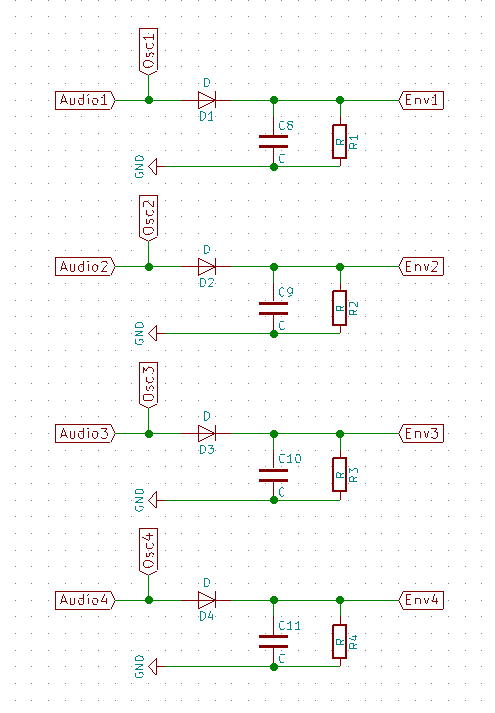
\includegraphics[width=0.5\textwidth, angle=0]{detektory.png}

    \caption{Schemat detektorów obwiedni}
 \label{fig-detektory}
    

\end{figure}

W tej sekcji zrealizowano również wyprowadzenie używane przy podłączeniu oscyloskopów (patrz rys. \ref{fig-oscyloskop}).
\begin{figure}[ht]

    \centering

  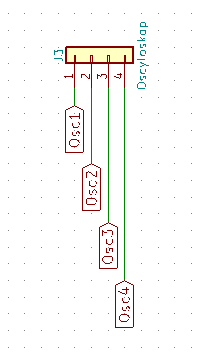
\includegraphics[width=0.15\textwidth, angle=0]{oscyloskop.png}

    \caption{Złącza testowe oscyloskopu}
 \label{fig-oscyloskop}
    

\end{figure}
\newpage

\subsection{Sekcja mikrokontrolera}
Mikrokontroler został zasilony napięciem 3.3V, dotakowo przy jego sekcji zasilania zastosowano filtry tak aby całkowicie wyeliminować wpływ ewentualnych tętnień na jego pracę (patrz rys. \ref{fig-filtry}).
\begin{figure}[ht]

    \centering

  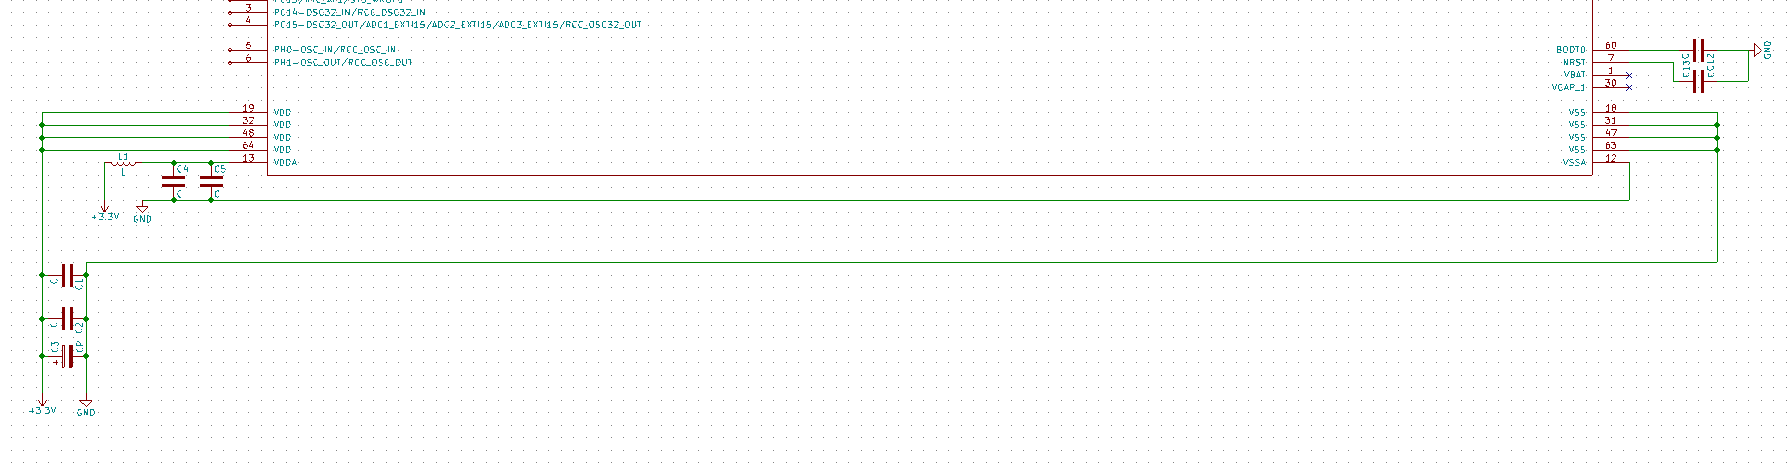
\includegraphics[width=1.1\textwidth, angle=0]{filtry.png}

    \caption{Zasilanie mikrokontrolera}
 \label{fig-filtry}
    

\end{figure}

Kolejną częścią tej sekcji jest podłączenie do przetwornika ADC mikrokontrolera sygnałów otrzymanych z generatora obwiedni oraz mikrofonów (patrz rys. \ref{fig-adc}).
\begin{figure}[ht]

    \centering

  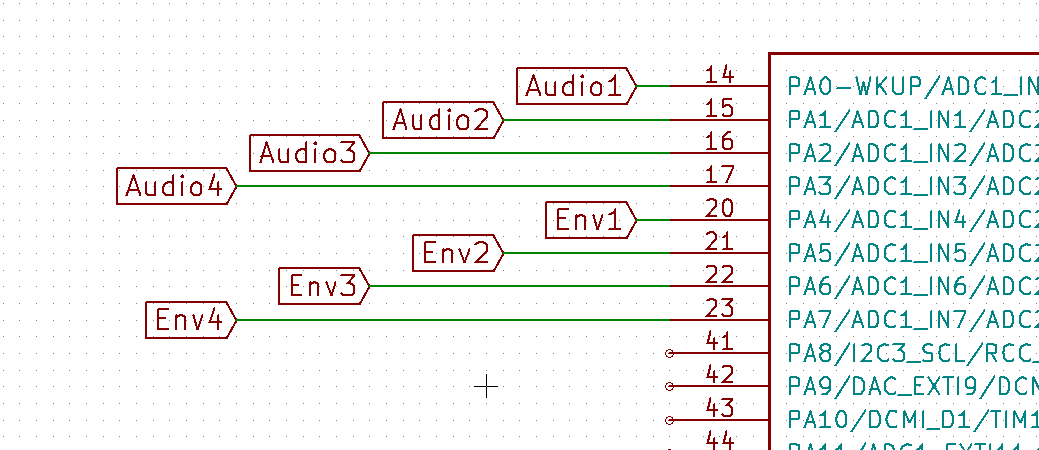
\includegraphics[width=0.6\textwidth, angle=0]{podlaczenie.png}

    \caption{Wejścia ADC}
 \label{fig-adc}
    

\end{figure}

Wyprowadzono także złącze programatora i interfejsu USART, służą one do programowania mikrokontrolera, debugowania za pomocą STM Studio i wysyłania danych testowych do komputera  (patrz rys. \ref{fig-programator}).
\begin{figure}[ht]

    \centering

  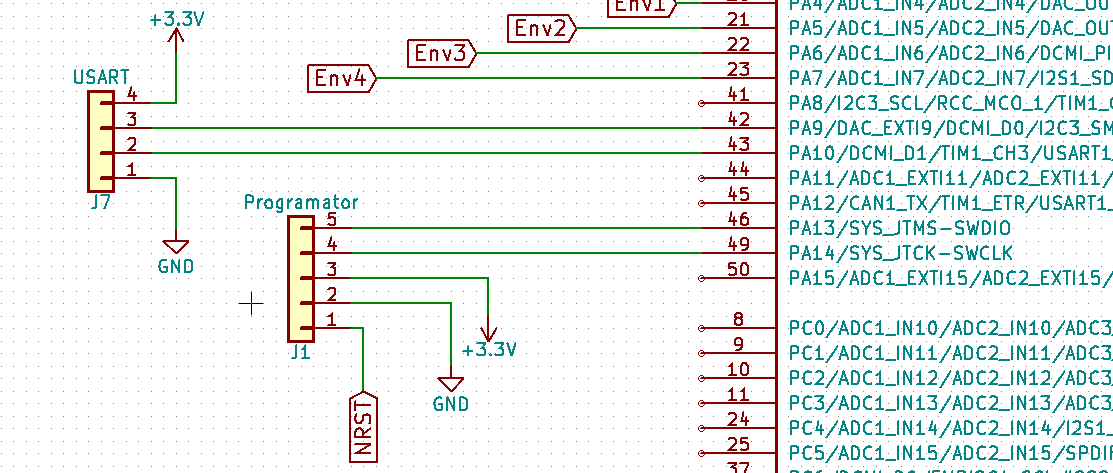
\includegraphics[width=0.6\textwidth, angle=0]{usart.png}

    \caption{Złącze programatora}
 \label{fig-programator}
    

\end{figure}

\chapter{Testy i eksperymenty}
\section{Testy mikrofonów i detektorów obwiedni}
W celu sprawdzenia poprawności działania układu, przeprowadzono testy działania mikrofonów oraz detektorów obwiedni. Do analizy sygnału użyto oscyloskopu. W pierwszej kolejności zbadano przebieg sygnału w ciszy, miało to na celu sprawdzenie w jakim stopniu szumy tła mogą wpłynąć na wyniki pomiarów.(patrz rys. \ref{fig-tlo}). Sygnał oznaczony kolorem zielonym jest wyjściem mikrofonu, natomiast kolorem pomarańczowym oznaczono wyjście detektora obwiedni. 
\begin{figure}[ht]

    \centering

  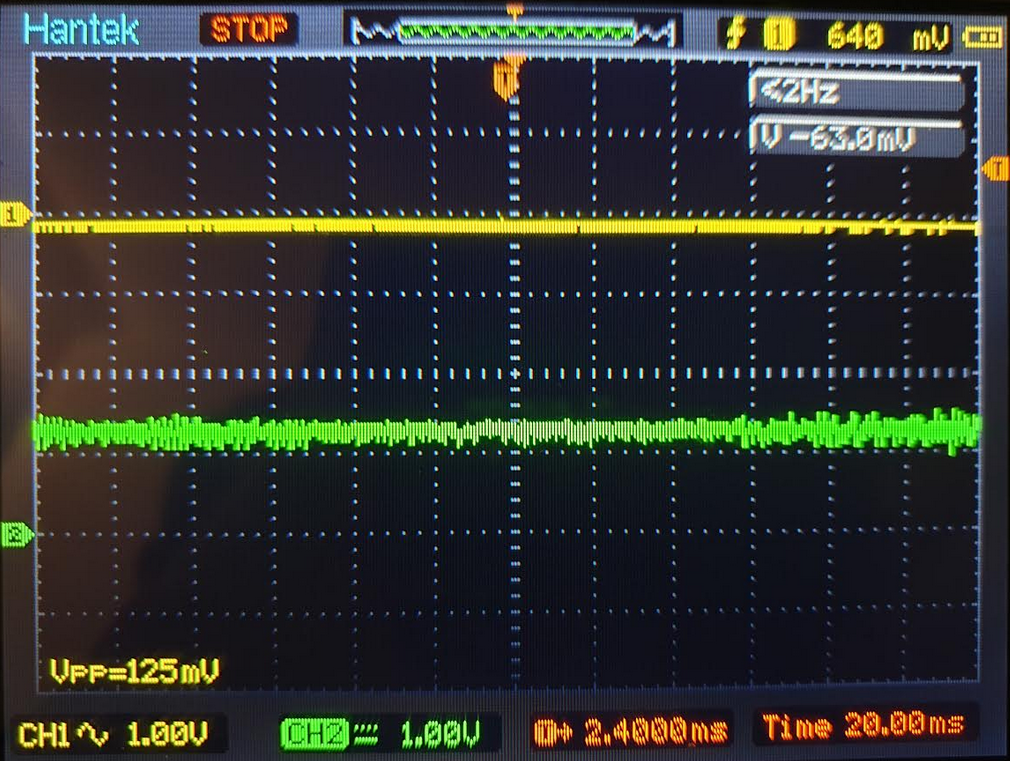
\includegraphics[width=0.7\textwidth, angle=0]{obwiednia_syg2.png}

    \caption{Szumy tła}
 \label{fig-tlo}
    

\end{figure}

Kolejnym krokiem było sprawdzenie poprawności działania detektora obwiedni, aby każda próba była powtarzalna nagrano dźwięk pstryknięcia palcami i odtwarzano go w równych odstępach czasu. Pierwsza próba dowiodła poprawności działania diody prostowniczej w układzie, jednak analizując przebieg można było dojść do wniosku, że filtr dolnoprzepustowy został źle dobrany, dlatego z każdą kolejną próbą zwiększano pojemność kondensatora aż do osiągnięcia satysfakconującego wyniku(patrz rys. \ref{fig-przebieg1}).

\begin{figure}[ht]

    \centering

  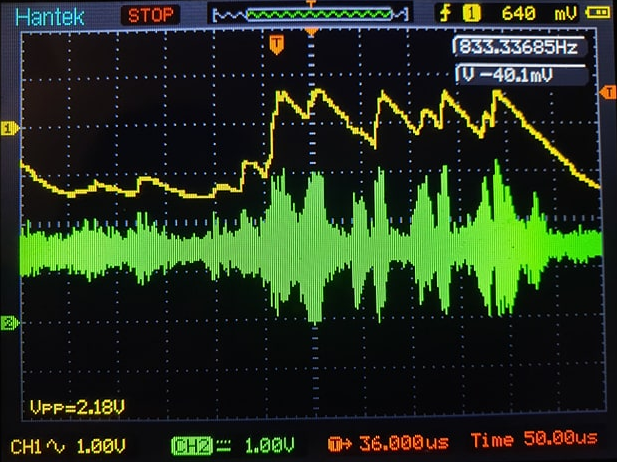
\includegraphics[width=0.7\textwidth, angle=0]{obwiednia_syg1.png}

    \caption{Pierwsza próba detektora obwiedni}
 \label{fig-przebieg1}
    

\end{figure}





\section{Testy działania programu}
Pierwsze testy działania programu zostały przeprowadzone bez podłączania systemu mikrofonów, miało to na celu sprawdzenie działania algorytmu w hermetycznym środowisku, dzięki takiemu działaniu można było założyć że wszystkie błędy wynikały z niepoprawnej implementacji Sum and Delay Bemaforming.
Na wejście algorytmu został podany sygnał o przebiegu trójkątnym (patrz rys.\ref{fig-sygnal}).
\begin{figure}[!ht]

    \centering

  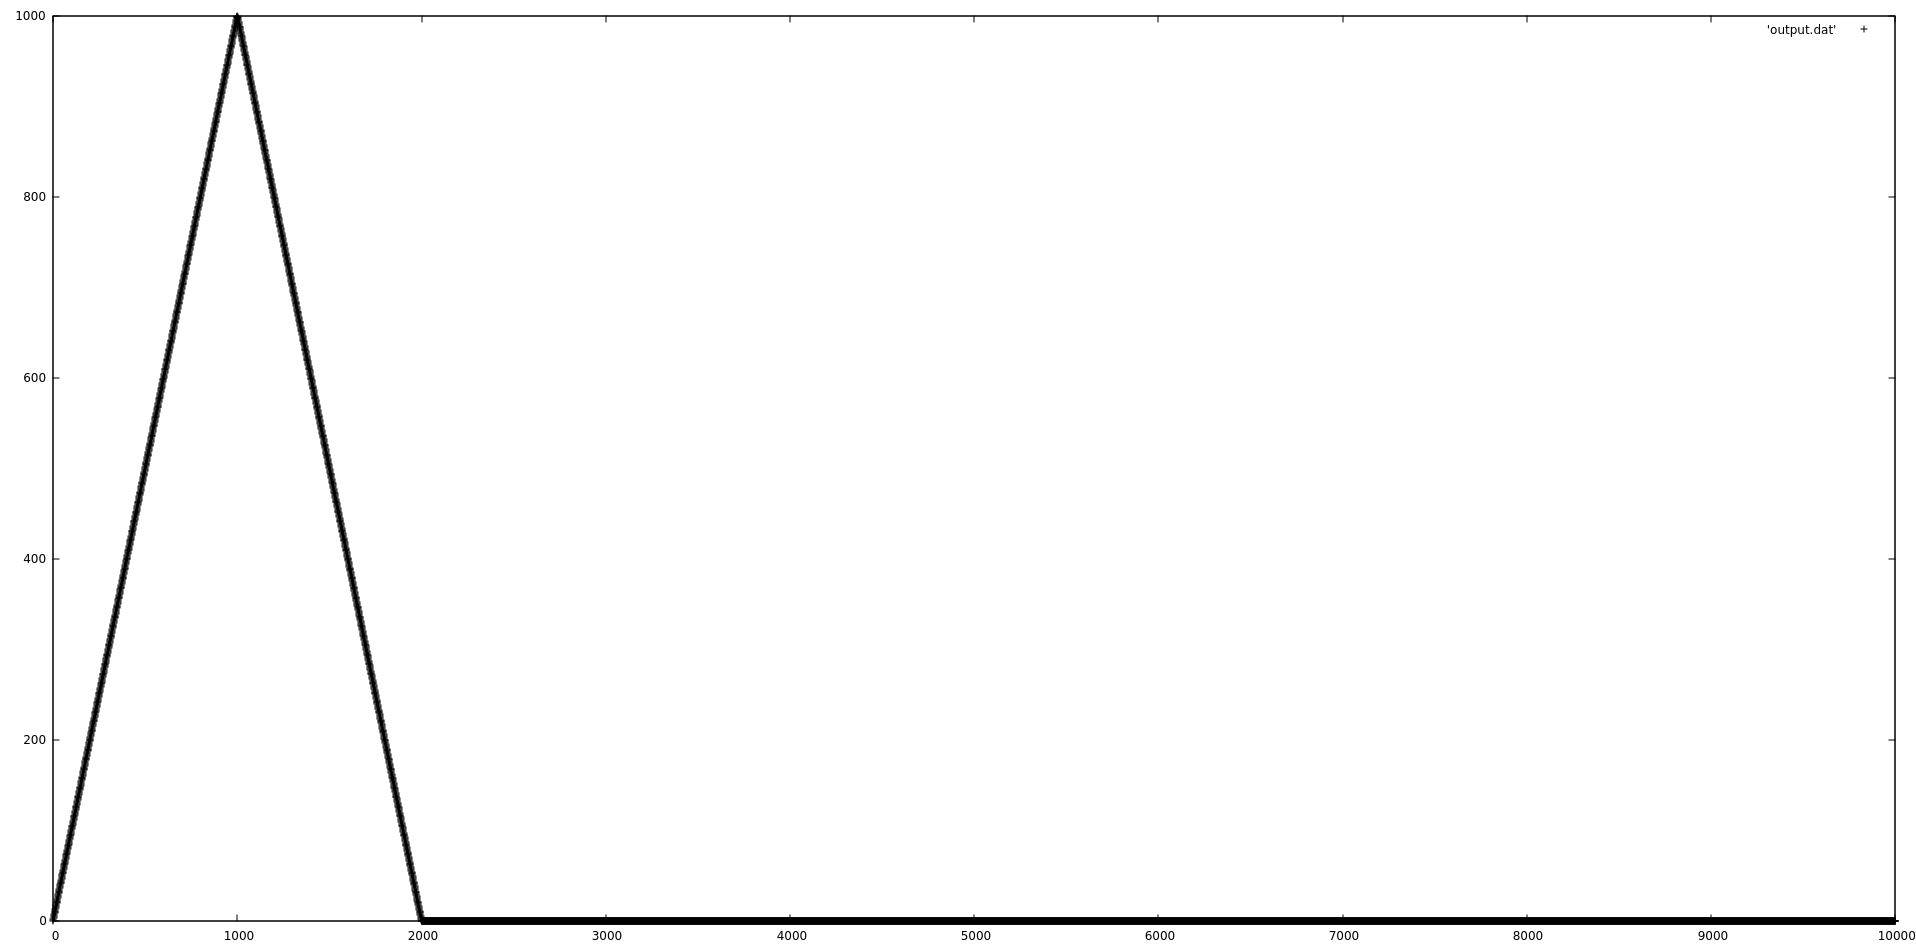
\includegraphics[width=1\textwidth, angle=0]{sygnal.png}

    \caption{Sygnał podany na wejście algorytmu}
 \label{fig-sygnal}
    

\end{figure}

\newpage

Założono że każdy z mikrofonów otrzymał ten sam sygnał który nie jest opóźniony, dla takich danych poprawnie działający algorytm powinien zwrócić maksymalną wartość korelacji w punkcie odpowiadającym kątowi 90 stopni. Wyniki eksperymentu można zaobserwować na poniższym wykresie
(patrz rys.\ref{fig-suma}). Wykres dowodzi poprawności działania programu, ponieważ widać na nim jak w miare zbliżania się watości kąta do 90 stopni rośnie wartość współczynnika korelacji.

\begin{figure}[!ht]

    \centering

  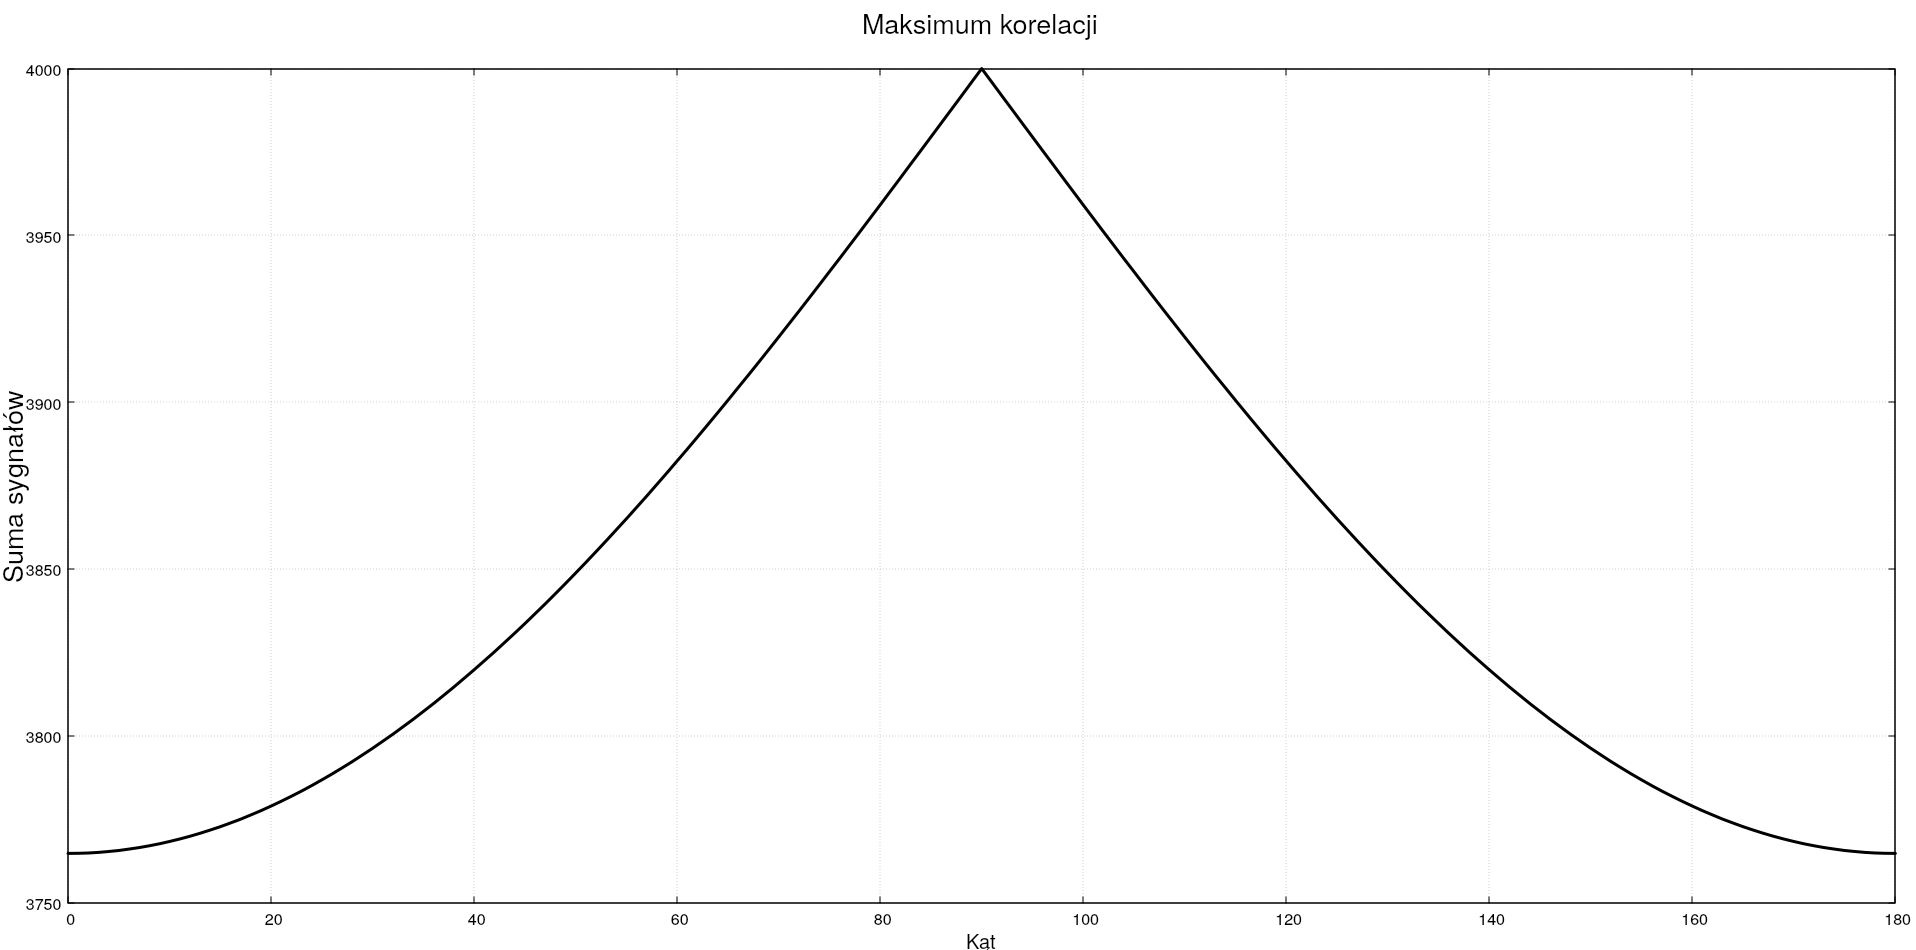
\includegraphics[width=1\textwidth, angle=0]{suma.png}

    \caption{Wartości korelacji}
 \label{fig-suma}
    

\end{figure}

%I=dt/T

Następnie, aby sprawdzić poprawność działania algorytmu dla sygnałów opóźnionych na wejście algorytmu podano cztery różne sygnały opóźnione w taki sposób aby symulowały kąt przybycia fali akustycznej równy 70 stopni. Dodatkowo aby upewnić się, że szumy otoczenia nie wpływają na wynik końcowy dodano do sygnału  zakłócenie którego opóźnienie sugeruje, że znajduję się on pod kątem 120 stopni względem matrycy (patrz rys.\ref{fig-opoznienia}). 

\begin{figure}[!ht]

    \centering

  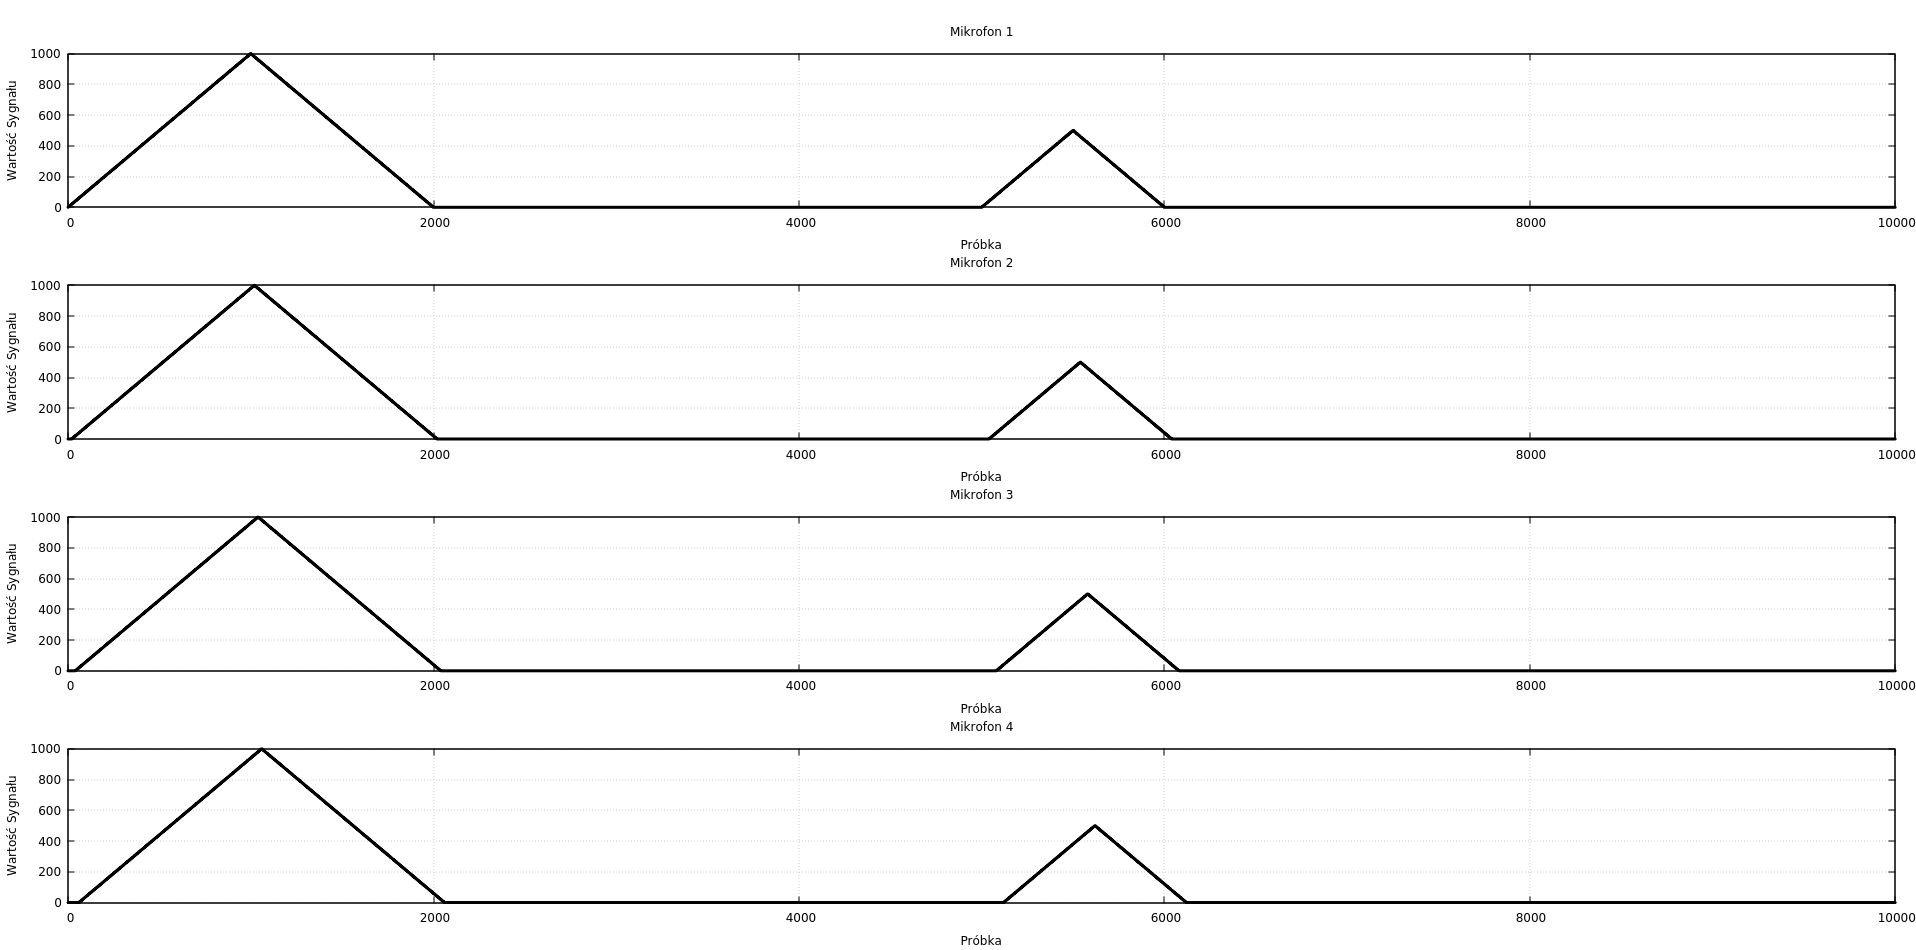
\includegraphics[width=0.9\textwidth, angle=0]{sygnaly.png}

    \caption{Symulowane sygnały}
 \label{fig-opoznienia}
    

\end{figure}

Wynikiem tego testu jest wykres korelacji sygnału, który potwierdza, że zaimplementowany algorytm Sum and Delay Beamforming działa poprawnie, ponieważ maksimum korelacji sygnałów odpowiada kątowi 70 stopni (patrz rys.\ref{fig-korelacja}). .

\begin{figure}[!ht]

    \centering

  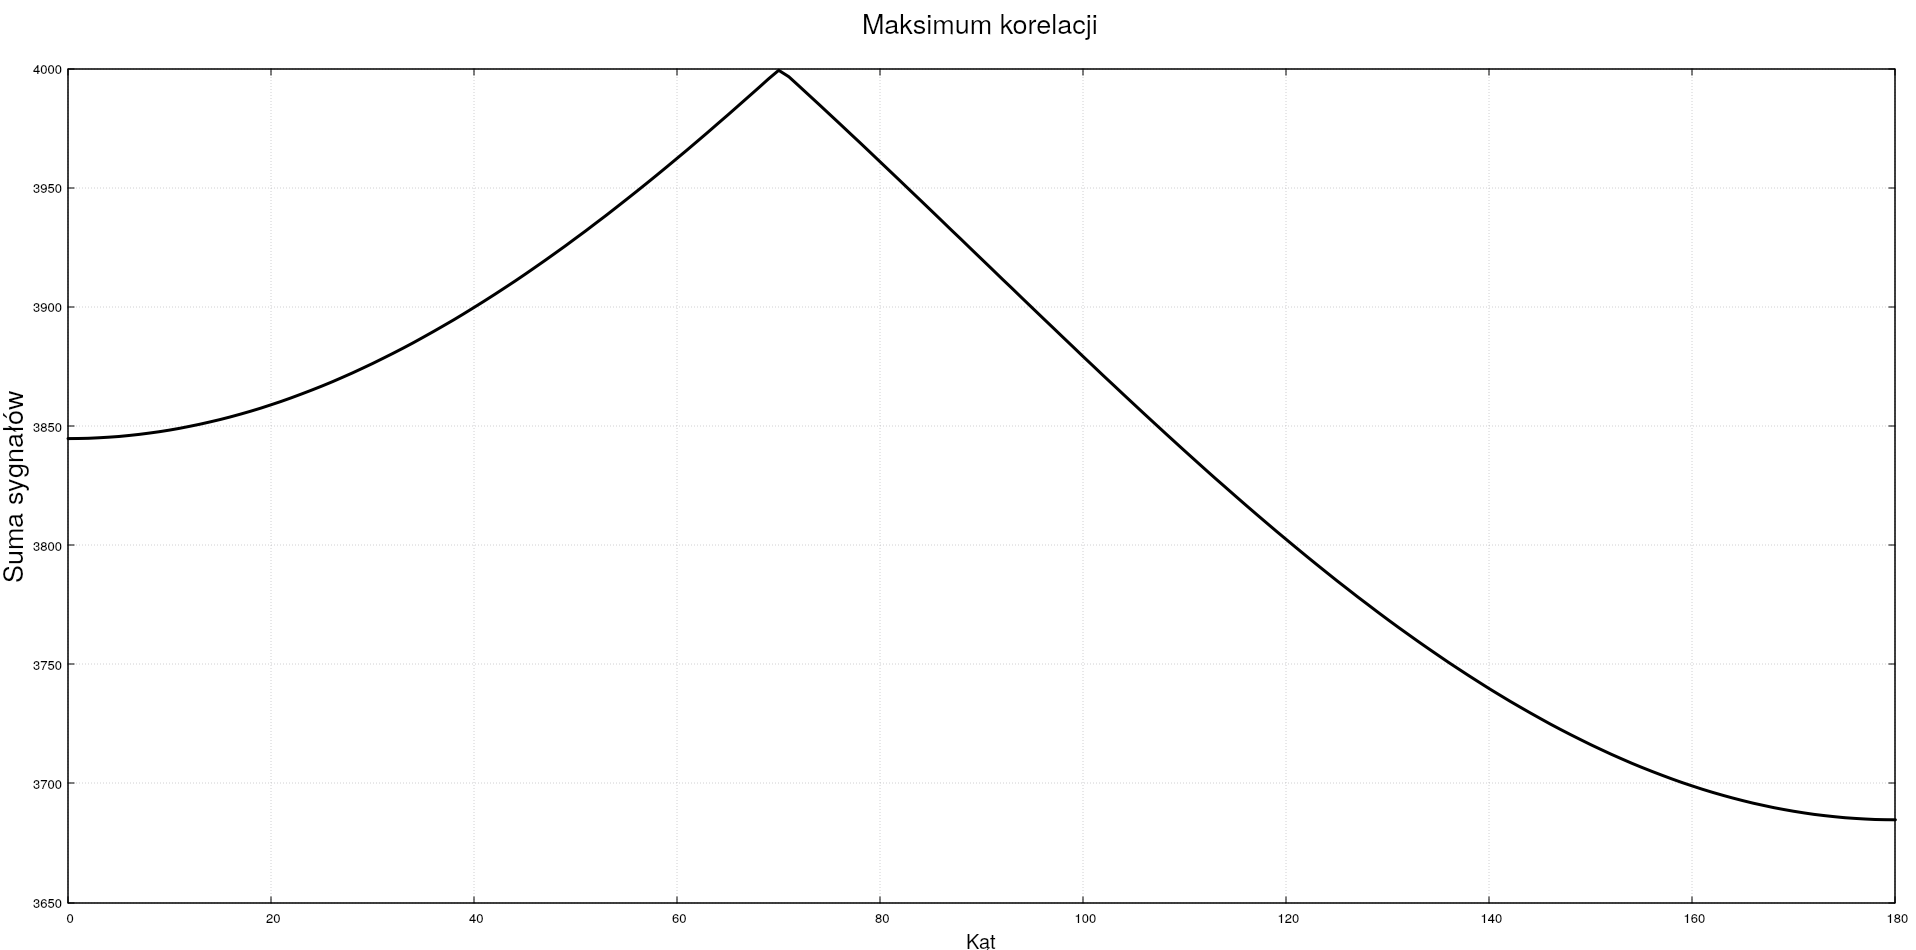
\includegraphics[width=0.9\textwidth, angle=0]{suma_opoznienie.png}

    \caption{Wartości korelacji dla sygnałów opóźnionych}
 \label{fig-korelacja}
    

\end{figure}
% \appendix tworzy dodatek

\addcontentsline{toc}{chapter}{\bibname} %utworzenie w spisie treści pozycji Literatura
\bibliography{bibliografia} % wstawia bibliografię korzystając z pliku bibliografia.bib - dotyczy BibTeXa, jeżeli nie korzystamy z BibTeXa należy użyć otoczenia thebibliography

%opcjonalnie może się tu pojawić spis rysunków i tabel
% \listoffigures
% \listoftables
\end{document}

